\documentclass[11pt]{article}
\usepackage{amsmath}
%\usepackage{extsizes}
\usepackage{amsmath,amssymb}
%\usepackage{omegavn,ocmrvn}
%\usepackage[utf8x]{inputenc}
\usepackage[utf8]{vietnam}

\usepackage{listings}
\lstset{language=Python}          % Set your language (you can change the language for each code-block optionally)


\usepackage{longtable}
\usepackage{answers}
\usepackage{graphicx}
\usepackage{array}
\usepackage{pifont}
\usepackage{picinpar}
\usepackage{enumerate}
\usepackage[top=3.0cm, bottom=3.5cm, left=3.5cm, right=2.5cm] {geometry}

\usepackage{extarrows}
\usepackage{hyperref}


\newtheorem{bt}{Câu}
\newcommand{\RR}{\mathbb R}
\Newassociation{sol}{Solution}{ans}
\newtheorem{ex}{Câu}
\renewcommand{\solutionstyle}[1]{\textbf{ #1}.}


\begin{document}
% \noindent

\begin{tabular*}
	{\linewidth}{c>{\centering\hspace{0pt}} p{.7\textwidth}}
	Trường ĐHKHTN, ĐHQGHN & {\bf Học Kỳ 2 (2021-2022)}
	\tabularnewline
	K64 TTƯD - Thầy Hà Phi & {\bf Bài Tập Giải Tích Số \\ \today}
	% Exercises on pages 239, 240 Cheney/Kincaid are really nice
	\tabularnewline
	\rule{1in}{1pt}  \small  & \rule{2in}{1pt} %(Due date:)
	\tabularnewline
	%  \tabularnewline
	%  &(Đề thi có 1 trang)
\end{tabular*}




\begin{center}
	{\bf Bài Tập Lý Thuyết Điều Khiển Hệ Thống - No. 3}
\end{center}

\begin{bt} Các hệ thống sau có điều khiển được hay không? Vì sao? Tìm hàm truyền của các hệ thống đó. (\textbf{Gợi ý: Xem lại Bài tập 4, phiếu Bài tập No.1.}) \\
a) \textbf{Dạng chính tắc điều khiển được (controllability canonical form)}
%
\begin{align}
	\dot{x} &= \m{0 & 1 & &  & \\ &  \ddots & \ddots &  & \\ & & \ddots & \ddots &   \\&  &  & 0 & 1 \\ -\a_1 & -\a_2 & \dots & \dots & -\a_{r} } x + \m{0 \\ \vdots \\ \vdots \\ 0 \\ 1} u, \\
y &= \m{\b_1 &  \dots & \dots & \b_r} x + D u, 
\end{align}
%
trong đó $\a_i$, $\b_i$, $D$ là các hệ số (thực hoặc phức). \\
b) \textbf{Dạng chính tắc quan sát được (observability canonical form)}
%
\begin{align}
	\dot{x} &= \m{-\a_1 & 1 & &  & \\ \vdots &   & \ddots &  & \\ \vdots & & & \ddots &   \\ -\a_{r-1} &  &  &  & 1 \\ -\a_{r} & 0 & \dots & \dots & 0} x + \m{\b_1 \\  \vdots \\ \vdots \\ \b_{r-1} \\ \b_r} u, \\
y &= \m{1 &  0 & \dots & \dots & 0} x + D u, 
\end{align}
%
trong đó $\a_i$, $\b_i$, $D$ là các hệ số (thực hoặc phức). \\
c) \textbf{Bài toán nhận dạng (relization problem): Cho trước hàm truyền, đi tìm dạng không gian trạng thái.} \\
Hãy tổng quát hóa các dạng chính tắc ở trên, sao cho hàm truyền của hệ có dạng 
%
\begin{equation}
	G(s) = D + \dfrac{\b_r s^{r-1} + \dots + \b_2 s + \b_1}{s^r + \a_r s^{r-1} + \dots + \a_{2} s + \a_1} \ ,
\end{equation}
%
trong đó $r \leq n$. Ở đây $G(s)$ được gọi là 1 hàm chính thường, \textbf{proper function}.
\end{bt}

\begin{bt} \textbf{Nghiên cứu về tính điều khiển được của 2 hệ thống được mắc nối tiếp/song song với nhau theo các sơ đồ trong Hình \ref{fig:electricalconnection}.} \\

\begin{figure}[!h]
	\centering
	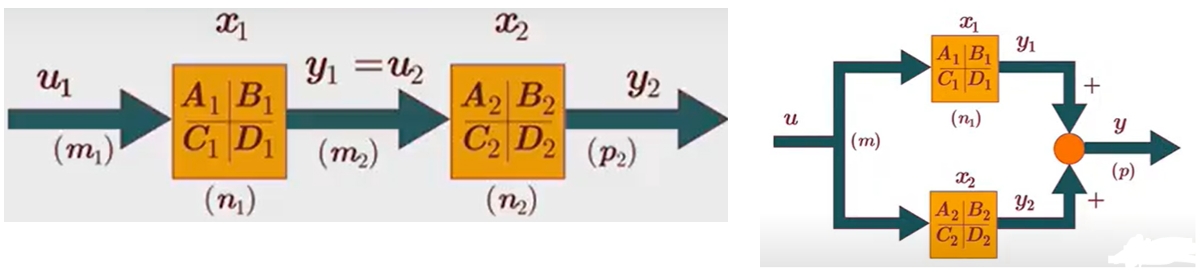
\includegraphics[scale = 0.6]{../Figures/Electrical_connection}
	\caption{Mạch nối tiếp (trái) \& Mạch song song (phải)}
	\label{fig:electricalconnection}
\end{figure}

\noindent Giả sử rằng các hệ con đều là điều khiển được. \\
1) Hãy xây dựng phương trình của hệ thống mắc nối tiếp, chú ý rằng ở đây đầu vào của hệ tổng chỉ có $u_1$, và đầu ra của hệ tổng là $y_2$. Chứng minh rằng nếu hệ thống tổng là điều khiển được thì nó không thể có vector riêng trái dạng $w = \m{w_1 & 0} \in \C^{n_1+n_2}$ mà thỏa mãn điều kiện $w^H B= 0$ . \\
2) Hãy xây dựng phương trình của hệ thống song song. Chứng minh hệ thống song song sẽ đánh mất tính điều khiển được khi và chỉ khi $A_1$ và $A_2$ có giá trị riêng chung $\lambda$, và các vector riêng trái $w_1$, $w_2$ tương ứng thỏa mãn
\begin{align*}
	& w^H_1 B_1 + w^H_2 B_2 = 0, \\
	& w^H_1 A_1 = \lambda w^H_1,   \   w^H_2 A_2 = \lambda w^H_2.
\end{align*}
\end{bt}


\begin{bt}
Cho hệ điều khiển LTI là SISO (single input/single output). Hãy chứng minh
công thức hàm truyền sau
%
\begin{equation}
G(s) := D+C(sI-A)^{-1}B \ \xlongequal{\text{chứng minh}} \ \dfrac{\det(sI-A+BC)}{\det(sI-A)}-1+D \ .  
\end{equation}
%
\end{bt}

\begin{bt}
Cho hệ thống điều khiển với thiết kế đạo hàm có dạng
%
\begin{align}
\dot{x} &= Ax+Bu, \\
y &= Cx, \\
z &= \dfrac{dy}{dt}
\end{align}
%
Hãy chuyển hệ trên về hệ điều khiển truyền thống, vẫn với đầu vào $u$ nhưng đầu ra là $z$.
\end{bt}	

\begin{bt}
a) Trong trường hợp hệ ổn định, Gramian điều khiển $W_c$ được xác định bởi công thức
%
\[
W_c  = \int_0^{\infty} e^{At} BB^T e^{A^Tt} dt. 
\]
%
Hãy chứng minh $W_c$ thỏa mãn phương trình Lyapunov sau
%
\begin{equation}\label{lyap}
	A W_c + W_c A^T = - B B^T \ .
\end{equation}
%
b) Trường hợp tổng quát của phương trình Lyapunov là phương trình Sylvester có dạng
%
\begin{equation}\label{sylvester}
A X + X B = C.
\end{equation}
%
Chứng minh rằng điều kiện cần và đủ để phương trình Sylvester có nghiệm là 
$\si(A) \cap \si(-B) = \emptyset$, trong đó $\si(A)$ là phổ của ma trận A. \\
c) \textbf{Luật khử Roth} \\
Chứng minh rằng điều kiện đủ để hai ma trận $\m{A & C\\0 & B}$ và $\m{A & 0 \\ 0 & B}$ (với số chiều ma trận phù hợp) là đồng dạng là \textbf{phương trình Sylvester $AX - XB = C$ có nghiệm}.
\end{bt}

\begin{bt} \textbf{Bài tập lập trình (Optional)} \\
	Hãy đi tìm hiểu các lệnh sau trong MATLAB: \textbf{ctrb, ctrbf}. Thực hành dựa trên: \\
	a) Bài tập 5a, phiếu Bài tập No.2. \\
	b) Ví dụ của Bài tập 1 ở trên (chon 2 vector $\alpha$ và $\beta$ là input vector). Viết function kiểm tra tính điều khiển được trong MATLAB. 
\end{bt}   

\begin{bt}
Chứng minh rằng hệ 
%
\begin{equation}
	\dot{x} = \m{A_{11} & A_{12} \\ A_{21} & A_{22}} x + \m{B_1 \\ 0} u,
\end{equation}
%
là điều khiển được thì cặp $(A_{22},A_{21})$ phải là điều khiển được.
\end{bt}

\begin{bt}
	Cho 2 hàm truyền của 2 hệ thống điều khiển mắc nối tiếp có dạng là
	%
	\begin{equation*}
		G_1(s) = \dfrac{2s+1}{s^2+2s+1} \ , \	G_2(s) = \dfrac{s^2+3s+2}{2s^2-s-1} \ . 
	\end{equation*}
	%
	a) Tìm hàm truyền của hệ thống tổng. \\
	b) Xây dựng mô hình không gian trạng thái của 2 hệ thống con sao cho cả 2 hệ thống con đó đều là điều khiển được. \\
	c) Hệ thống tổng có điều khiển được không? Vì sao? \\
	d) Trình bày ý tưởng tìm phân tích điều khiển Kalman và rút gọn hệ thống tổng
	nếu nó không điều khiển được.
\end{bt}

\begin{bt}
	Cho 2 hàm truyền của 2 hệ thống điều khiển mắc nối tiếp có dạng là
	%
	\begin{equation*}
		G_1(s) = \dfrac{2s+1}{s^2+2s+1} \ , \	G_2(s) = \dfrac{s^2+3s+2}{2s^2-s-1} \ . 
	\end{equation*}
	%
	a) Tìm hàm truyền của hệ thống tổng. \\
	b) Xây dựng mô hình không gian trạng thái của 2 hệ thống con sao cho cả 2 hệ thống con đó đều là quan sát được. \\
	c) Hệ thống tổng có quan sát được không? Vì sao? \\
	d) Trình bày ý tưởng tìm phân tích quan sát Kalman và rút gọn hệ thống tổng
	nếu nó không quan sát được.
\end{bt}
	
\end{document}



